% $Header$

\documentclass{beamer}

% This file is a solution template for:

% - Giving a talk on some subject.
% - The talk is between 15min and 45min long.
% - Style is ornate.



% Copyright 2004 by Till Tantau <tantau@users.sourceforge.net>.
%
% In principle, this file can be redistributed and/or modified under
% the terms of the GNU Public License, version 2.
%
% However, this file is supposed to be a template to be modified
% for your own needs. For this reason, if you use this file as a
% template and not specifically distribute it as part of a another
% package/program, I grant the extra permission to freely copy and
% modify this file as you see fit and even to delete this copyright
% notice.


\mode<presentation>
{
  %\usetheme{whale}%{Berlin}%{Warsaw}
  % or ...

  \setbeamercovered{transparent}
  % or whatever (possibly just delete it)
}


\usepackage[english]{babel}
% or whatever

\usepackage{graphicx}

\usepackage[latin1]{inputenc}
% or whatever

\usepackage{times}
\usepackage[T1]{fontenc}
% Or whatever. Note that the encoding and the font should match. If T1
% does not look nice, try deleting the line with the fontenc.



\title%[Short Paper Title] % (optional, use only with long paper titles)
{Interpretable asset markets}

%\subtitle
%{Presentation Subtitle} % (optional)

\author%[Author] % (optional, use only with lots of authors)
{Gao Qinghui}
% - Use the \inst{?} command only if the authors have different
%   affiliation.

\institute%[Universities of Somewhere and Elsewhere] % (optional, but mostly needed)
{
  Wang Yanan Institute for Studies in Economics (WISE)

  Xiamen University
}
% - Use the \inst command only if there are several affiliations.
% - Keep it simple, no one is interested in your street address.

\date%[Short Occasion] % (optional)
{\today  }

\subject{Talks}
% This is only inserted into the PDF information catalog. Can be left
% out.



% If you have a file called "university-logo-filename.xxx", where xxx
% is a graphic format that can be processed by latex or pdflatex,
% resp., then you can add a logo as follows:

% \pgfdeclareimage[height=0.5cm]{university-logo}{university-logo-filename}
% \logo{\pgfuseimage{university-logo}}



% Delete this, if you do not want the table of contents to pop up at
% the beginning of each subsection:
%\AtBeginSubsection[]
%{
%  \begin{frame}<beamer>{Overview}
%    \tableofcontents[currentsection,currentsubsection]
%  \end{frame}
%}


% If you wish to uncover everything in a step-wise fashion, uncomment
% the following command:

%\beamerdefaultoverlayspecification{<+->}


\begin{document}



\begin{frame}
  \titlepage
\end{frame}

%\setbeamertemplate{headline}{}

\begin{frame}{Outline}
  \tableofcontents%[pausesections]
  % You might wish to add the option [pausesections]
\end{frame}


% Since this a solution template for a generic talk, very little can
% be said about how it should be structured. However, the talk length
% of between 15min and 45min and the theme suggest that you stick to
% the following rules:

% - Exactly two or three sections (other than the summary).
% - At *most* three subsections per section.
% - Talk about 30s to 2min per frame. So there should be between about
%   15 and 30 frames, all told.

\section{Motivation}

\begin{frame}{Motivation}
    \begin{itemize}
    \item An often discussed but not verified view: The \textbf{aggregate economic uncertainty} has sizable effects on \textbf{asset valuations} and financial markets \textbf{dislike economic uncertainty}.
    \item  Information regarding future expected growth might be encoded in current asset valuation.
    \end{itemize}
\end{frame}

%\subsection%[Short First Subsection Name]
%{First Subsection Name}



%\begin{frame}{Make Titles Informative. Use Uppercase Letters.}{Subtitles are optional.}
%  % - A title should summarize the slide in an understandable fashion
%  %   for anyone how does not follow everything on the slide itself.
%
%  \begin{itemize}
%  \item
%    Use \texttt{itemize} a lot.
%  \item
%    Use very short sentences or short phrases.
%  \end{itemize}
%\end{frame}

%\begin{frame}{Make Titles Informative.}
%
%  You can create overlays\dots
%  \begin{itemize}
%  \item using the \texttt{pause} command:
%    \begin{itemize}
%    \item
%      First item.
%      \pause
%    \item
%      Second item.
%    \end{itemize}
%  \item
%    using overlay specifications:
%    \begin{itemize}
%    \item<3->
%      First item.
%    \item<4->
%      Second item.
%    \end{itemize}
%  \item
%    using the general \texttt{uncover} command:
%    \begin{itemize}
%      \uncover<5->{\item
%        First item.}
%      \uncover<6->{\item
%        Second item.}
%    \end{itemize}
%  \end{itemize}
%\end{frame}


%\subsection{Second Subsection}
%
%\begin{frame}{Make Titles Informative.}
%\end{frame}
%
%\begin{frame}{Make Titles Informative.}
%\end{frame}

\section{Literature Review}

\begin{frame}{Literature Review}

\begin{itemize}
    \item
    A rise in economic uncertainty increases expected returns and leads to a fall in asset valuations. A rise in expected growth, on the other hand leads to a rise in asset valuations. Both these effects can be interpreted from the perspective of general equilibrium models (e.g., Bansal and Yaron, 2004).

    \item
    Asset markets "shuts-off" the channels of expected growth rates and economic uncertainty, as growth rates are assumed to be i.i.d. (e.g., Campbell and Cochrane, 1999; Cechetti et al., 2000).

\end{itemize}

\end{frame}

\section{Framework and Approach}

\begin{frame}{The economy and asset valuation}
\scriptsize
    \begin{itemize}
    \item
        Using the Campbell and Shiller(1988) approximation to write the log valuation ratio.
        \begin{eqnarray}
            p_t - y_t = \kappa_t + E_t \sum^{\infty}_{j=1} \kappa_{1}^j [ g_{y,t+j} - r_{t+j}]
        \end{eqnarray}

        where $p_t$ is the log of the stock price, $y_t$ is the log-level of cash-flows, $g_{y,t+1}$ is the growth rate of market cash-flows, and $r_{t+1}$ is the continuously compounded return on the market portfolio.

    \item
        An additional accounting implication of the above present value restriction is:
        \begin{eqnarray}
            var(p_t - y_t) = \sum_{j=1}^{\infty} \kappa_{1}^j [ cov(g_{y,t+j} - y_t)
        \end{eqnarray}
    \end{itemize}
\end{frame}

\begin{frame}{The economy and asset valuation (Cont'd)}
    \begin{itemize}
    \item
        Following this intuition, the main focus of this paper is in exploring
        the links between fundamental economic uncertainty and asset valuation. Consider
        the following projections:
        \begin{eqnarray}
            E_t[r_{t+1}] = r_f + \gamma \sigma^2_{c,t}
        \end{eqnarray}

        where $\gamma$ capture attitudes toward risk governed by preferences and technology in the economy Substituting the expression for expected returns is Eq. (3) into Eq. (1)
        implies that a rise in anticipated consumption volatility should lower asset
        valuations, $p_t - y_t$.
        \end{itemize}
\end{frame}

\begin{frame}{The economy and asset valuation (Cont'd)}
    \begin{itemize}
    \item
        In a variety of models, expected returns are determined by the conditional volatility of aggregate consumption, that is
        \begin{eqnarray}
            p_t - y_t = b_0 + b_\sigma \sigma_{c,t-1} + u_{1,t}
        \end{eqnarray}

        where $\sigma_{c,t-1}$ ia a measure of consumption volatility as of time $t -1$. A negative $b_\sigma$ in the above projection indicates that financial markets dislike economic uncertainty.
        \end{itemize}
\end{frame}

\begin{frame}{The economy and asset valuation (Cont'd)}

\scriptsize
    \begin{itemize}
    \item
        substituting the expression for the expected returns (Eq. (3)) into Eq. (2). If consumption volatility is time varying and is important for explaining expected returns then $p_t - y_t$ should also predict \textit{future} consumption volatility. Hence, consider the following additional projection:
        \begin{eqnarray}
            | \eta_{c, t+J} | = \alpha_0 + \alpha_{1,J} (p_t - y_t)  + u_{2,t+J}, \qquad J \leq 1
        \end{eqnarray}

        where $|\eta_{c, t+J}|$ is the one step-ahead innovation in the consumption growth at date t + J. If volatility is long-lasting then current valuation rations should be able to predict future realized consumption volatility, and $\alpha_{1,J}$ should be different from zero. Further, if financial markets dislike economic uncertainty, and the volatility process is persistent, then $\alpha_{1,J}$ should be negative as well.
        \end{itemize}
\end{frame}

\begin{frame}{Approach and Findings}

\begin{enumerate}
  \item regressing $p_t - y_t$ on to $\sigma_{c,t-1}$ produces sizeable negative slope coefficients and significant $R^2$s
  \item future (realized) economic uncertainty, $|\eta_{c,t+J}|$ is predicted by $p_t - y_t$, with negative slope coefficients
  \item current $p_t - y_t$ predicts future growth rates, $g_{y, t+J}$, with a positive slope coefficient.
\end{enumerate}

Data: quarterly data of US spanning the period 1949.1-1999.4 (from CRSP and NIPA)
%%    \begin{itemize}
%%    \item
%%        substituting the expression for the expected returns (Eq. (3)) into Eq. (2). If consumption volatility is time varying and is important for explaining expected returns then $p_t - y_t$ should also predict \textit{future} consumption volatility. Hence, consider the following additional projection:
%%        \begin{eqnarray}
%%            | \eta_{c, t+J} | = \alpha_0 + \alpha_{1,J} (p_t - y_t)  + u_{2,t+J}, \qquad J \leq 1
%%        \end{eqnarray}
%%
%%        where $|\eta_{c, t+J}|$ is the one step-ahead innovation in the consumption growth at date t + J. If volatility is long-lasting then current valuation rations should be able to predict future realized consumption volatility, and $\alpha_{1,J}$ should be different from zero. Further, if financial markets dislike economic uncertainty, and the volatility process is persistent, then $\alpha_{1,J}$ should be negative as well.
%%        \end{itemize}
\end{frame}


\section{Empirical Evidence - Volatility implications}

\begin{frame}{Summary Statistics: USA(quarterly)}
\tiny
\begin{table}
\centering
\caption{Summary Statistics: USA (quarterly)}
\label{my-label}
\begin{tabular}{lllcrr}
\hline
                                                                 &  $E(\cdot)$     &  $\sigma(\cdot)$     &  $corr(g_c, g_{\cdot})$    &    $AC(4)$    &   $AC(8)$     \\ \hline
USA(1949.1 - 1999.2)                                             &       &       &      &        &        \\
$g_c$                                                               & 0.008 & 0.005 &      & 0.009  & -0.128 \\
$g_d$                                                               & 0.005 & 0.017 & 0.11 & -0.037 & -0.023 \\
$g_e$                                                               & 0.002 & 0.068 & 0.31 & -0.094 & -0.159 \\
$r_m$                                                               & 0.021 & 0.078 &      & 0.002  & -0.032 \\
$(p-d)$                                                              & 3.333 & 0.317 &      & 0.768  & 0.594  \\
$((p-e)$                                                              & 2.203 & 0.422 &      & 0.781  & 0.576  \\
\\
\begin{tabular}[c]{@{}l@{}}USA(1972.1 - 1998.2)\end{tabular} &       &       &      &        &        \\
$g_c$                                                               & 0.007 & 0.005 &      & 0.034  & -0.194 \\
$g_d$                                                               & 0.004 & 0.015 & 0.16 & -0.183 & 0.078  \\
$g_e$                                                               & 0.004 & 0.064 & 0.32 & 0.054  & -0.257 \\
$r_m$                                                               & 0.019 & 0.082 &      & -0.016 & -0.029 \\
$(p-d)$                                                              & 3.340  & 0.295 &     & 0.680   & 0.496  \\
$(p-e)$                                                              & 2.247 & 0.343 &      & 0.706  & 0.509  \\ \hline
                                                                % &       &       &      &        &
\end{tabular}
\end{table}
$g_c$, $g_d$, and $g_e$ deonote respectively the real growth rate of consumption, dividends, and earings. $r_m$ is the real return on the market portfolio. $p-d$ and $p-e$ denote the log price-dividend and price-earnings, respectively. $E(\cdot)$ and $\sigma(\cdot)$ denote the mean and standard deviation, and $AC(j)$ is the $j$th autocorrelation.


\end{frame}

%\begin{frame}
%\tiny
%\begin{table}[]
%\centering
%\caption{Summary Statistics: USA (quarterly) (Copied)}
%\label{my-label}
%\begin{tabular}{lrrcrr}
%\hline
%&  $E(\cdot)$     &  $\sigma(\cdot)$     &  $corr(g_c, g_{\cdot})$    &    $AC(4)$    &   $AC(8)$     \\ \hline
%USA(1949.1 - 1999.2) &         &        &        &         &         \\
%$g_c$                   & 0.0087  & 0.0050  &        & -0.0244 & -0.1237 \\
%$g_d$                   & 0.0053  & 0.0202 & 0.1019 & -0.0083 & 0.0194  \\
%$g_e$                   & 0.0019  & 0.0766 & 0.1059 & -0.0844 & -0.0772 \\
%$r_m$                   & 0.0216  & 0.0777 &        & -0.0250  & -0.0285 \\
%$(p-d)$                  & 4.7083  & 0.3018 &        & 0.7467  & 0.562   \\
%$(p-e)$                  & 16.0950  & 0.3521 &        & 0.7181  & 0.5349  \\
%USA(1972.1 - 1998.2) &         &        &        &         &         \\
%$g_c$                   & 0.0075  & 0.0043 &        & 0.0382  & -0.1226 \\
%$g_d$                   & 0.0045  & 0.0144 & 0.1728 & -0.1413 & 0.1178  \\
%$g_e$                   & 0.0034  & 0.0741 & 0.2481 & -0.0737 & -0.1352 \\
%$(r_m)$                   & 0.0193  & 0.0833 &        & -0.0170  & -0.0086 \\
%$(p-d)$                  & 4.7078  & 0.2825 &        & 0.6665  & 0.5340   \\
%$(p-e)$                  & 16.1848 & 0.2781 &        & 0.6626  & 0.4588 \\ \hline
%\end{tabular}
%\end{table}
%
%\end{frame}

\subsection{Consumption Dynamics and volatility}




\begin{frame}{Two Measures of Economic Uncertainty}

Two Measures of Economic Uncertainty

\begin{enumerate}
    \item
    $\sigma_{c,t-1,J} = log( \sum_{j=1}^{J} |\eta_{c, t-j}|)$  (Anderson et al. 2003)
    \\where $\eta_{c,t}$ is the innovation in consumption growth.

    \item
    $\sigma_{c,t}$ which is based on modelling consumption growth as following an AR(1)-GARCH(1,1).

\end{enumerate}
\end{frame}

\begin{frame}{regression models}

\begin{itemize}
    \item
        \begin{eqnarray}
             g_{c,t} = \mu + A_1 g_{c, t-1}  + \eta_{c,t}
        \end{eqnarray}

    \item

               \[g_{c,t} = \mu + A_1 g_{c, t-1}  + \eta_{c,t} \]
        \begin{eqnarray}
                \sigma_{c,t}^2 = \omega_0 + \omega_{c,t-1}^2 + \omega_2 \sigma_{c,t-1}^2
        \end{eqnarray}

\end{itemize}
\end{frame}



\begin{frame}{Consumption growth and market return projection (quarterly)}
\tiny

\begin{table}
\centering
\caption{\footnotesize Consumption growth and market return projection (quarterly) }
\label{my-label}
\begin{tabular}{rrrrrrrrrr}
\hline
%                      & \multicolumn{3}{c}{Growth rates/returns}             &            &            &          & \multicolumn{2}{c}{Absolute residuals} &         \\ \cline{2-6} \cline{8-10}
                      & $\mu$                    & $A_1$     & $\omega_0$    & $\omega_1$ & $\omega_2$ &          & AC(1)             & AC(4)              & AC(8)   \\ \hline
\multicolumn{3}{l}{$AR(1)$ estimates}                      &               &            &            &          &                   &                    &         \\ \cline{1-3}
\multicolumn{3}{l}{Panel A: Consumption growth}             &               &            &            &          &                   &                    &         \\
Estimate              & 0.007                    & 0.234    &               &            &            & Estimate & 0.174            & 0.088            & 0.049 \\
S.E.                  & 0.001                 & 0.080    &               &            &            & Q-stat   & 6.20            & 17.73            & 30.76 \\
                      &                          &           &               &            &            &          &                   &                    &         \\
\multicolumn{3}{l}{Panel B: Market return}                  &               &            &            &          &                   &                    &         \\
Estimate              & 0.020                    & 0.066     &               &            &            & Estimate & 0.108            & 0.071             & -0.083 \\
S.E.                  & 0.006                   & 0.079   &               &            &            & Q-stat   & 2.39            & 9.61              & 16.20 \\
                      &                          &           &               &            &            &          &                   &                    &         \\
                      \cline{1-3}
\multicolumn{3}{l}{\textit{AR(1)-GARCH(1,1) estimates}}            &               &            &            &          &                   &                    &   \\
\cline{1-3}
\multicolumn{3}{l}{Panel C: Consumption growth}             &               &            &            &          &                   &                    &         \\
Estimate              & 0.007                    & 0.310    & 1.63*      & 0.143     & 0.788     &          &                   &                    &         \\
S.E.                  & 0.001                 & 0.076    & 1.68*      & 0.073     & 0.091     &          &                   &                    &         \\
                      &                          &           &               &            &            &          &                   &                    &         \\
\multicolumn{3}{l}{Panel D: Market return}                  &               &            &            &          &                   &                    &         \\
Estimate              & 0.002                   & 0.090    & 0.002         & 0.139     & 0.541     &          &                   &                    &         \\
S.E.                  & 0.006                   & 0.078    & 0.001        & 0.118     & 0.166     &          &                   &                    &   \\ \hline
\end{tabular}
\end{table}


\end{frame}


%\begin{frame}{Consumption growth and market return projection (quarterly)}
%\tiny
%
%\begin{table}
%\centering
%\caption{\footnotesize Consumption growth and market return projection (quarterly) (copied)}
%\label{my-label}
%\begin{tabular}{rrrrrrrrrr}
%\hline
%%                      & \multicolumn{3}{c}{Growth rates/returns}             &            &            &          & \multicolumn{2}{c}{Absolute residuals} &         \\ \cline{2-6} \cline{8-10}
%                      & $\mu$                    & $A_1$     & $\omega_0$    & $\omega_1$ & $\omega_2$ &          & AC(1)             & AC(4)              & AC(8)   \\ \hline
%\multicolumn{3}{l}{$AR(1)$ estimates}                      &               &            &            &          &                   &                    &         \\ \cline{1-3}
%\multicolumn{3}{l}{Panel A: Consumption growth}             &               &            &            &          &                   &                    &         \\
%Estimate              & 0.0070                    & 0.1956    &               &            &            & Estimate & 0.2104            & 0.0663             & -0.0031 \\
%S.E.                  & 5.26E-04                 & 0.0531    &               &            &            & Q-stat   & 9.0284            & 19.3894            & 32.8089 \\
%                      &                          &           &               &            &            &          &                   &                    &         \\
%\multicolumn{3}{l}{Panel B: Market return}                  &               &            &            &          &                   &                    &         \\
%Estimate              & 0.0200                     & 0.0780     &               &            &            & Estimate & 0.1152            & 0.0581             & -0.0798 \\
%S.E.                  & 0.0062                   & 0.0649    &               &            &            & Q-stat   & 2.7066            & 9.4510              & 16.0491 \\
%                      &                          &           &               &            &            &          &                   &                    &         \\
%                      \cline{1-3}
%\multicolumn{3}{l}{\textit{AR(1)-GARCH(1,1) estimates}}            &               &            &            &          &                   &                    &   \\
%\cline{1-3}
%\multicolumn{3}{l}{Panel C: Consumption growth}             &               &            &            &          &                   &                    &         \\
%Estimate              & 0.0070                    & 0.1945    & 1.39E-05      & 0.2973     & 0.1279     &          &                   &                    &         \\
%S.E.                  & 8.31E-04                 & 0.0842    & 4.15E-06      & 0.1153     & 0.2375     &          &                   &                    &         \\
%                      &                          &           &               &            &            &          &                   &                    &         \\
%\multicolumn{3}{l}{Panel D: Market return}                  &               &            &            &          &                   &                    &         \\
%Estimate              & 0.0194                   & 0.1011    & 0.0020         & 0.1412     & 0.5253     &          &                   &                    &         \\
%S.E.                  & 0.0065                   & 0.0936    & 0.0014        & 0.0815     & 0.2815     &          &                   &                    &   \\ \hline
%\end{tabular}
%\end{table}
%\end{frame}

\subsection{Economic uncertainty and asset valuations}

%\begin{frame}
%\tiny
%\begin{table}[]
%\centering
%\caption{My caption}
%\label{my-label}
%\begin{tabular}{llllllllllllll}
%\hline
%J   & \multicolumn{6}{l}{Regressor $\sigma_{c,t-1,J}$}                                          &  & \multicolumn{6}{l}{Regressor $\sigma_{r_m,t-1,J}$}                                   \\ \cline{2-7} \cline{9-14}
%    & \multicolumn{3}{l}{Data}                    & \multicolumn{3}{l}{Monte-Carlo}             &  & \multicolumn{3}{l}{Data}               & \multicolumn{3}{l}{Monte-Carlo}             \\ \hline
%    & $b_{\sigma, J}$   & t-stat   & $\bar{R}^2$  & $t(2.5\%)$ & $t(2.5\%)$ & $\bar{R}^2(95\%)$ &  & $b_{\sigma, J}$ & t-stat & $\bar{R}^2$ & $t(2.5\%)$ & $t(2.5\%)$ & $\bar{R}^2(95\%)$ \\ \cline{1-4}
%\multicolumn{4}{l}{Panel A: Price�Cdividend ratio} &            &            &                   &  &                 &        &             &            &            &                   \\ \cline{1-4}
%1   & -0.084            & -2.614   & 0.08         & -1.870     & -1.496     & 0.04              &  & -0.049          & -2.274 & 0.03        & -1.546     & -1.232     & 0.02              \\
%4   & -0.254            & -3.703   & 0.19         & -3.873     & -3.197     & 0.16              &  & -0.088          & -1.275 & 0.02        & -2.733     & -2.266     & 0.09              \\
%8   & -0.358            & -3.153   & 0.26         & -4.024     & -3.256     & 0.25              &  & -0.135          & -1.348 & 0.03        & -2.998     & -2.474     & 0.16              \\
%    &                   &          &              &            &            &                   &  &                 &        &             &            &            &                   \\ \cline{1-4}
%\multicolumn{4}{l}{Panel B: Price�Cearnings ratio} &            &            &                   &  &                 &        &             &            &            &                   \\ \cline{1-4}
%1   & -0.111            & -2.428   & 0.08         & -1.826     & -1.435     & 0.04              &  & -0.026          & -0.446 & 0.00        & -1.521     & -1.214     & 0.02              \\
%4   & -0.364            & -4.053   & 0.23         & -3.708     & -3.047     & 0.15              &  & -0.000          & -0.001 & 0.00        & -2.669     & -2.268     & 0.08              \\
%8   & -0.489            & -4.398   & 0.33         & -3.778     & -3.111     & 0.23              &  & -0.019          & -0.150 & 0.00        & -2.913     & -2.430     & 0.14              \\ \hline
%\end{tabular}
%\end{table}
%\end{frame}

\begin{frame}{Economic uncertainty predicting future valuation ratios: USA}
\small
\[
    p_t - y_t = b_0 + b_{\sigma,J} \sigma_{c,t-1,J} + \mu_{1,t}
\]

\tiny
\begin{table}[]
\centering
\caption{Economic uncertainty predicting future valuation ratios: USA}
\label{my-label}
\begin{tabular}{lllllll}
\hline
J   & \multicolumn{6}{l}{Regressor $\sigma_{c,t-1,J}$}                                          \\ \cline{2-7}
    & \multicolumn{3}{l}{Data}                    & \multicolumn{3}{l}{Monte-Carlo}             \\ \hline
    & $b_{\sigma, J}$   & t-stat   & $\bar{R}^2$  & $t(2.5\%)$ & $t(2.5\%)$ & $\bar{R}^2(95\%)$ \\ \hline
Panel A: Price dividend ratio &   & & &         &            &                   \\ \cline{1-1}
1   & -0.084            & -2.614   & 0.08         & -1.870     & -1.496     & 0.04              \\
4   & -0.254            & -3.703   & 0.19         & -3.873     & -3.197     & 0.16              \\
8   & -0.358            & -3.153   & 0.26         & -4.024     & -3.256     & 0.25              \\
    &                   &          &              &            &            &                   \\ \hline
Panel B: Price earnings ratio &     & & &       &            &                   \\ \cline{1-1}
1   & -0.111            & -2.428   & 0.08         & -1.826     & -1.435     & 0.04              \\
4   & -0.364            & -4.053   & 0.23         & -3.708     & -3.047     & 0.15              \\
8   & -0.489            & -4.398   & 0.33         & -3.778     & -3.111     & 0.23              \\ \hline
\end{tabular}
\end{table}
\end{frame}

\begin{frame}{Economic uncertainty predicting future valuation ratios: USA}
\small
\[
    p_t - y_t = b_0 + b_{\sigma,J} \sigma_{r_m,t-1,J} + \mu_{1,t}
\]

\tiny

\begin{table}[]

\centering
\caption{Economic uncertainty predicting future valuation ratios: USA}
\label{my-label}
\begin{tabular}{lllllll}
\hline
J                             & \multicolumn{6}{l}{Regressor $\sigma_{r_m,t-1,J}$}                                   \\ \cline{2-7}
                              & \multicolumn{3}{l}{Data}               & \multicolumn{3}{l}{Monte-Carlo}             \\ \hline
                              & $b_{\sigma, J}$ & t-stat & $\bar{R}^2$ & $t(2.5\%)$ & $t(2.5\%)$ & $\bar{R}^2(95\%)$ \\ \hline
Panel A: Price dividend ratio &                 &        &             &            &            &                   \\ \cline{1-1}
1                             & -0.049          & -2.274 & 0.03        & -1.546     & -1.232     & 0.02              \\
4                             & -0.088          & -1.275 & 0.02        & -2.733     & -2.266     & 0.09              \\
8                             & -0.135          & -1.348 & 0.03        & -2.998     & -2.474     & 0.16              \\
                              &                 &        &             &            &            &                   \\ \hline
Panel B: Price earnings ratio &                 &        &             &            &            &                   \\ \cline{1-1}
1                             & -0.026          & -0.446 & 0.00        & -1.521     & -1.214     & 0.02              \\
4                             & -0.000          & -0.001 & 0.00        & -2.669     & -2.268     & 0.08              \\
8                             & -0.019          & -0.150 & 0.00        & -2.913     & -2.430     & 0.14              \\ \hline
\end{tabular}
\end{table}
\end{frame}


\subsection{Valuation ratios predict economic uncertainty}




\begin{frame}{PICTURE}

Left: $\sigma_{c,t-1,12}$ versus $(p_t-e_t)$ \\
Right: $e_t - e_{t-12}$ versus $p_t - e_t$ \\

All variables are standardized.

\begin{figure}
  \centering
  % Requires \usepackage{graphicx}
  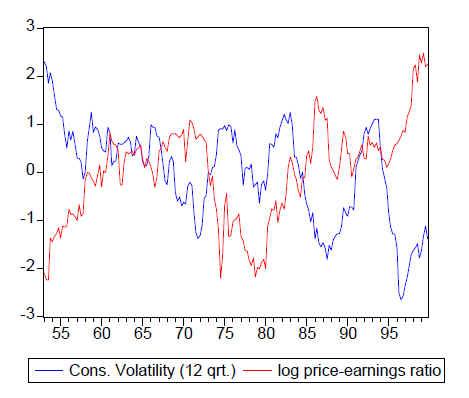
\includegraphics[width=5cm]{figure1.png} 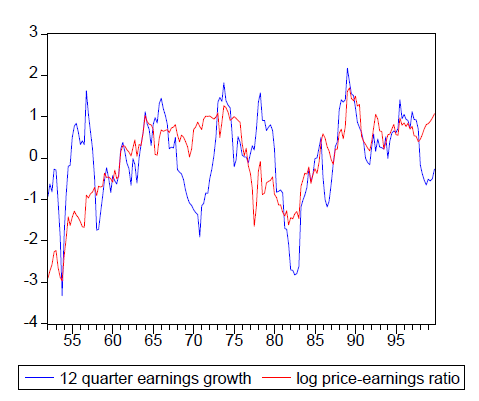
\includegraphics[width=5cm]{figure2.png}\\
  \caption{Fig.1}%\label{}
\end{figure}
\end{frame}

\begin{frame}{Valuation ratios predicting future economic uncertainty: USA}
\tiny
\begin{table}[]
\centering
\caption{Valuation ratios predicting future economic uncertainty: USA}
\label{Valuation ratios predicting future economic uncertainty: USA}
\begin{tabular}{lllllll}
\hline
J                             & \multicolumn{6}{l}{Predicting $|\eta_{c, t+J}|$}                                       \\ \cline{2-7}
                              & \multicolumn{3}{l}{Data}                 & \multicolumn{3}{l}{Monte-Carlo}             \\ \hline
                              & $\alpha_{1, J}$ & t-stat    & $\bar{R}^2$ & $t(2.5\%)$ & $t(2.5\%)$ & $\bar{R}^2(95\%)$ \\ \cline{1-1}
Panel A: Price dividend ratio &                &           &             &            &            &                   \\ \cline{1-1}
1                             & -1.012         & -4.027    & 0.08        & -3.200     & -2.661     & 0.04              \\
4                             & -0.788         & -3.064    & 0.04        & -3.059     & -2.553     & 0.04              \\
8                             & -0.796         & -3.13     & 0.04        & -3.035     & -2.501     & 0.04              \\
                              &                &           &             &            &            &                   \\ \cline{1-1}
Panel B: Price earnings ratio &                &           &             &            &            &                   \\ \cline{1-1}
1                             & -0.806         & -4.899    & 0.1         & -3.121     & -2.602     & 0.04              \\
4                             & -0.629         & -3.772    & 0.05        & -3.066     & -2.53      & 0.04              \\
8                             & -0.594         & -3.59     & 0.04        & -3.062     & -2.518     & 0.04              \\ \hline
\end{tabular}
\end{table}
\end{frame}


\begin{frame}{Valuation ratios predicting future economic uncertainty: USA}
\tiny
\begin{table}[]
\centering
\caption{Valuation ratios predicting future economic uncertainty: USA}
\label{my-label}
\begin{tabular}{lllllll}
\hline
J                             & \multicolumn{6}{l}{Predicting $|\eta_{r_m, t+J}|$}                                  \\ \cline{2-7}
                              & \multicolumn{3}{l}{Data}              & \multicolumn{3}{l}{Monte-Carlo}             \\ \hline
                              & $\alpha_{1, J}$ & t-stat & $\bar{R}^2$ & $t(2.5\%)$ & $t(2.5\%)$ & $\bar{R}^2(95\%)$ \\ \cline{1-1}
Panel A: Price dividend ratio &                &        &             &            &            &                   \\ \cline{1-1}
1                             & -0.592         & -1.760 & 0.02        & -2.322     & -1.929     & 0.02              \\
4                             & -0.194         & -0.549 & 0.00        & -2.353     & -1.935     & 0.02              \\
8                             & 0.117          & 0.330  & 0.00        & -2.434     & -1.997     & 0.02              \\
                              &                &        &             &            &            &                   \\ \cline{1-1}
Panel B: Price earnings ratio &                &        &             &            &            &                   \\ \cline{1-1}
1                             & -0.154         & -0.713 & 0.00        & -2.378     & -1.976     & 0.02              \\
4                             & -0.034         & -0.154 & 0.00        & -2.392     & -1.985     & 0.02              \\
8                             & -0.017         & -0.087 & 0.00        & -2.465     & -2.053     & 0.02              \\ \hline
\end{tabular}
\end{table}
\end{frame}


\subsection{GARCH consumption volatility and robustness}

\begin{frame}{regression function}

To account for the persistence is variables we also include distributed lags of the dependent variable in our projections.

\begin{itemize}
    \item
    \begin{eqnarray}
        p_t - e_t = \alpha_{1,0}  + \alpha_{1,1} (p_{t-1} - e_{t-1}) + \alpha_{1,2} log \sigma_{c,t-1}^2 + \epsilon_{1,t}
    \end{eqnarray}

    \item

    \begin{eqnarray}
        log \sigma_{c,t}^2  = \alpha_{2,0}  + \alpha_{2,1} (p_{t-1} - e_{t-1}) + \alpha_{2,2} log \sigma_{c,t-1}^2 + \epsilon_{2,t}
    \end{eqnarray}

\end{itemize}
\end{frame}


\begin{frame}{Price - earnings ratios and economic uncertainty: USA}
\tiny
\begin{table}[]
\centering
\caption{Price - earnings ratios and economic uncertainty: USA}
\label{my-label}
\begin{tabular}{llllllll}
\hline
                                   & \multicolumn{3}{l}{Data}                                                               & \multicolumn{4}{l}{Monte-Carlo}                                        \\ \cline{2-8}
                                   & Est.                       & t-stat                     & $\bar{R}^2$                   & $t(2.5\%)$        & $t(5\%)$ & $\bar{R}^2(95\%)$ & $\bar{R}^2(97.5\%)$ \\ \hline
\multicolumn{4}{l}{Panel A: Predicting price earnings ratio}                                                                &                   &          &                   &                     \\
\multicolumn{4}{l}{$p_t - e_t = \alpha_0,+ \alpha_1 log \sigma_{c,t-1}^2 + \epsilon_t$}                                     &                   &          &                   &                     \\
$\alpha_1$                         & -0.503                     & -5.08                     & 0.34                          & -2.93             & -2.4     & 0.22              & 0.28                \\
                                   &                            &                           &                               &                   &          &                   &                     \\
\multicolumn{5}{l}{$p_t - e_t = \alpha_{1,0},+ \alpha_{1,1} (p_{t-1} - e_{t-1}) + \alpha_{1,2} log \sigma_{c,t-1}^2 + \epsilon_{1,t}$}          &          &                   &                     \\
$\alpha_{1,2}$                     & -0.035                     & -2.08                     & 0.94                          & -1.78             & -1.5     & 0.96              & 0.97                \\
$\alpha_{1,1}$                     & 0.937                      & 40.32                     &                               &                   &          &                   &                     \\
                                   &                            &                           &                               &                   &          &                   &                     \\
\multicolumn{3}{l}{Panel B: Predicting volatility}                                          &                               &                   &          &                   &                     \\
\multicolumn{4}{l}{$log \sigma_{c,t}^2,= \alpha_0,+ \alpha_2 (p_{t-1}  - e_{t-1}) + \epsilon_t$}                            &                   &          &                   &                     \\
$\alpha_2$                         & -0.705                     & -4.6                      & 0.36                          & -2.45             & -2.05    & 0.23              & 0.29                \\
                                   &                            &                           &                               &                   &          &                   &                     \\
\multicolumn{5}{l}{$log \sigma_{c,t}^2,= \alpha_{2,0},+ \alpha_{2,1} (p_{t-1} - e_{t-1}) + \alpha_{2,2} log \sigma_{c,t-1}^2 + \epsilon_{2,t}$} &          &                   &                     \\
$\alpha_{2,1}$                     & -0.128                     & -2.95                     & 0.84                          & -1.55             & -1.34    & 0.93              & 0.94                \\
$\alpha_{2,2}$                     & 0.856                      & 26.67                     &                               &                   &          &                   &                     \\ \hline
\end{tabular}
\end{table}
\end{frame}

\section{Additional implications and empirical evidence}

\subsection{Growth rate and return predictability}

\begin{frame}{Two  predictability projection}

Growth-rate predictability projection:

\begin{eqnarray}
    \sum_{l=1}^L g_{y,t+l} = \beta_0 + \beta_{1,L} (p_t - y_t)  + u_{t+L}, \qquad L\leq 1,
\end{eqnarray}

and the companion return projection

\begin{eqnarray}
    \sum_{l=1}^L r_t+l = \beta_0 + \beta_{1,L} (p_t - y_t)  + u_{t+L}, \qquad L\leq 1.
\end{eqnarray}

\end{frame}

\begin{frame}{Valuation ratios predicting future growth rates and returns: USA}
\tiny
\begin{table}[]
\centering
\caption{Valuation ratios predicting future growth rates and returns: USA}
\label{my-label}
\begin{tabular}{llllllllllll}
\hline
$J$ & \multicolumn{3}{l}{Predicting $\sum_{l=1}^L g_{c,t+l}$} &  & \multicolumn{3}{l}{Predicting $\sum_{l=1}^L g_{d,t+l}$} &  & \multicolumn{3}{l}{Predicting $\sum_{l=1}^L r_{m,t+l}$} \\ \cline{2-4} \cline{6-8} \cline{10-12}
    & $\beta_{1,J}$       & $t-stat$       & $\bar{R}^2$      &  & $\beta_{1,J}$       & $t-stat$       & $\bar{R}^2$      &  & $\beta_{1,J}$       & $t-stat$       & $\bar{R}^2$      \\ \hline
\multicolumn{4}{l}{Panel A: Price dividend ratio}             &  &                     &                &                  &  &                     &                &                  \\
4   & 0.059               & 0.802          & 0.01             &  & 0.001               & 0.0540         & 0.00             &  & -0.139              & -2.071         & 0.06             \\
8   & 0.120               & 0.819          & 0.02             &  & -0.015              & -0.462         & 0.00             &  & -0.256              & -2.102         & 0.11             \\
12  & 0.237               & 1.366          & 0.07             &  & -0.041              & -1.327         & 0.01             &  & -0.366              & -1.931         & 0.15             \\
16  & 0.325               & 1.333          & 0.11             &  & -0.084              & -1.941         & 0.03             &  & -0.494              & -1.846         & 0.20             \\
\multicolumn{4}{l}{Panel B: Price earnings ratio}             &  &                     &                &                  &  &                     &                &                  \\
4   & 0.095               & 1.485          & 0.06             &  & -0.017              & -0.971         & 0.01             &  & -0.074              & -1.533         & 0.03             \\
8   & 0.195               & 1.650          & 0.14             &  & -0.027              & -0.937         & 0.01             &  & -0.149              & -1.646         & 0.07             \\
12  & 0.287               & 2.284          & 0.23             &  & -0.036              & -1.31          & 0.02             &  & -0.195              & -1.521         & 0.09             \\
16  & 0.350               & 2.071          & 0.31             &  & -0.058              & -1.649         & 0.04             &  & -0.272              & -1.586         & 0.15             \\ \hline
\end{tabular}
\end{table}
\end{frame}

\begin{frame}{Valuation ratios predicting future growth rates and returns}

Our main point is that, empirically, dividends behave very differently from earnings.
The results for predicting dividend growth (middle columns) replicate what is found
in the literature��that is dividend growth is not predictable by price�Cdividend ratios.
This is also true for trying to predict dividend growth using price�Cearnings ratio.
Earnings growth, however, is predicted by price�Cdividend ratios, and in a sizable and
significant manner by price�Cearnings ratios (left columns).

\end{frame}


\begin{frame}{Price - earnings ratio and growth rates}
\tiny
\begin{table}[]
\centering
\caption{Price - earnings ratio and growth rates}
\label{my-label}
\begin{tabular}{lllllllll}
\hline
$J$          & \multicolumn{3}{l}{Data}                                         &  & \multicolumn{3}{l}{Monte Carlo}     &                   \\ \cline{2-4} \cline{6-9}
             & $\beta_{1,J}$          & $t-stat$          & $\bar{R}^2$         &  & $t(90\%)$ & $t(95\%)$ & $t(97.5\%)$ & $\bar{R}^2(95\%)$ \\ \hline
\multicolumn{4}{l}{$sum_{l=1}^L g_{e,t+l} = \beta_0 + \beta_{1,L} (p_t - e_t)$} &  &           &           &             &                   \\
4            & 0.095                  & 1.485             & 0.06                &  & 1.609     & 2.033     & 2.425       & 0.07              \\
8            & 0.195                  & 1.65              & 0.14                &  & 1.638     & 2.115     & 2.506       & 0.13              \\
12           & 0.287                  & 2.284             & 0.23                &  & 1.733     & 2.194     & 2.615       & 0.2               \\
16           & 0.35                   & 2.071             & 0.31                &  & 1.79      & 2.274     & 2.709       & 0.27              \\ \hline
\end{tabular}
\end{table}

For each horizon, these $R^2$ are significantly smaller than the corresponding $R^2s$
for predicting future earnings growth. A common view, driven by the focus on
price $-$ dividend ratios, is that fluctuations in cost of capital and not in cash flows are
the key for explaining fluctuations in asset valuations. In fact, Cochrane (1992) and
Campbell and Cochrane (1999) advocate that about 100\% (or more) of the
fluctuations in price�Cdividend ratios are attributable to cost of capital.

\end{frame}





\section{Conclusion}

\begin{frame}{Conclusion}

  % Keep the summary *very short*.
%  \begin{itemize}
%  \item
%    The \alert{first main message} of your talk in one or two lines.
%  \item
%    The \alert{second main message} of your talk in one or two lines.
%  \item
%    Perhaps a \alert{third message}, but not more than that.
%  \end{itemize}

In this paper we show that measures of economic uncertainty (conditional
volatility of consumption) predicts and is predicted by valuation ratios at long
horizons. We show that asset valuations drop as economic uncertainty rises that is,
financial markets dislike economic uncertainty. Moreover, long horizon $R^2s$ from
predicting future economic growth (earnings growth) are fairly high for the US
price earnings ratios.

  % The following outlook is optional.
 % \vskip0pt plus.5fill
%  \begin{itemize}
%  \item
%    Outlook
%    \begin{itemize}
%    \item
%      Something you haven't solved.
%    \item
%      Something else you haven't solved.
%    \end{itemize}
%  \end{itemize}
\end{frame}


\end{document}


